\documentclass{article}

% Code
\usepackage{minted}

% Figures
\usepackage{graphicx} % Allows figures
\usepackage{caption}
\usepackage{subcaption}

% Math
\usepackage{amsmath}

% Section style
\usepackage{etoolbox} % for configuration of sloppy
\usepackage{xcolor}


\definecolor{secnum}{RGB}{102,102,102}

\makeatletter
    \def\@seccntformat#1{\llap{\color{secnum}\csname the#1\endcsname\hskip 16pt}}
\makeatother
%end section style

{\sloppy}{\hbadness 10000\relax}{}{} %adds hbadness to sloppy
{\sloppy}{\hbadness 0\relax}{}{} %adds hbadness to sloppy
\setlength{\paperheight}{297mm} %Sets the page to an A4
\setlength{\paperwidth}{210mm}        %Sets the page to an A4

\begin{document}

\begin{titlepage}
\begin{center}
\textsc{Introduction to Graphics}\\[0.5cm]
\textsc{Final Assignment: Parametric Surfaces}\\[0.5cm]
\vspace{2 cm}
\begin{tabular}{ll}
Student: & Kasper Passov\\
\end{tabular}
\end{center}
\vspace{5 cm}
\newpage
\end{titlepage}


\section{Parametric surfaces Implementation}
I have had very little success getting this to work, as the next few pages will show.

\subsection{Creating Patches}
To parse the patches from the data files into \texttt{BeizerPatch} data i used the ReadBezierPatches
and saved it into a vector of \texttt{BezierPatch}.
\begin{minted}{cpp}
    std::vector<BezierPatch> patches;
    ReadBezierPatches("data/teapot.data", patches);
\end{minted}
I then iterate over the patches, initializing each patches buffers.
\begin{minted}{cpp}
for (int i = 0; i < patches.size(); i++){
    GLPatch patch;
    patch.initializeBuffers(triangleShaderProgram, patches.at(i));
    buffers.push_back(patch);
\end{minted}
After the calculations of the perspective and shading each patch
is drawn by calling the \texttt{draw()} function, and then swapping
to the new drawn on buffer.
\begin{minted}{cpp}
for (int i = 0; i < buffers.size(); i++)[
    buffers.at(i).draw();
    }
glutSwapBuffers();
\end{minted}

\subsection{BezierPatch formating}
I chose to save the patch values in a list of floats, that is created
much like i created with an algorithm much like the subdivision algorithm
in the previous assignment. It splits the patch into subpatches until it
does not pass the flatnesstest, then it adds every point into the float list,
using a helper algorithm i created. 

\subsection{Results}
I created a few tests to find that the lists in each patch is filling out, but i am
unable to find the points in my world. This made me move my PRP closer to the points where
the teapot should be located and i discovered that one of the patches was being drawn, as
shown on figure \ref{fig:wat}.
\begin{figure}[h!]
\centering
    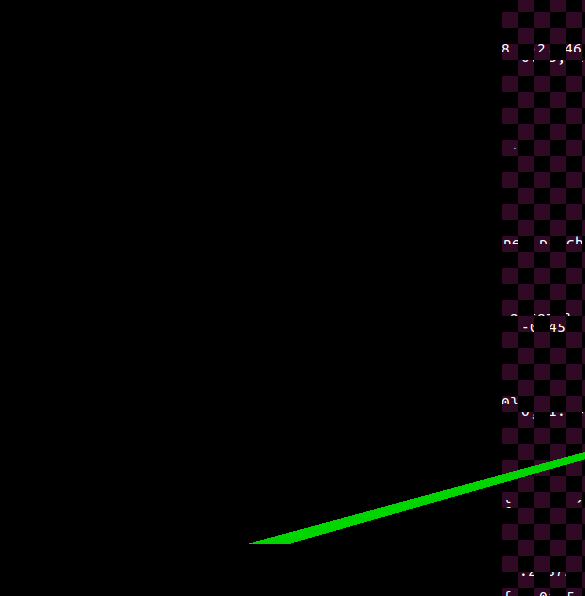
\includegraphics[width=0.5\textwidth, keepaspectratio]{wat.png}
    \caption{A teapot patch}
    \label{fig:wat}
\end{figure}\\
I also discovered the patch was only being drawn on some runs of the program. This makes
me belive i am doing something very wrong as that should not be right. My first though is
i missunderstod the way the patches are being drawn, so i should not create a new
instance of the GLPatch class everytime i wish to create a new patch. If this is the case
the reason for the shown patch are only sometimes drawn, could be the program picking one
of the initialized GLPatches and drawing that on the buffer, repeating this with new buffers
and new patches without saving the old.\\
I belive this to be a my mistake as i know it is possible for the code to draw one patch,
as i used the same code to draw the triangles shown below on figure \ref{fig:phongshade}.

\subsection{Late thoughts}
It is currently a little to late to make as widespreading changes as
this demands. But i belive i know where i am going wrong, unfortuantly i ran out of time
before i could get a working version.
I should only be creating one GLPatch and save all the patches values inside of this one 
patch, instead of the current implementation where i have a buffer for each patch. This would allow the program to draw everything on
the buffer before swapping it into view. 
Implementing this would mean removing all the BezierPatches code from the main only leaving
patch as a global variable in the file, this is left so i can do an init and a draw call on it when needed.
I would still need to calculate the Phong constants and perspective matrix in the main.cpp file.
\begin{minted}{cpp}
static void intializeShadersAndGLObjects() {
    ...
    patch.initializeBuffers(triangleShaderProgram);}

static void renderSceneCB() {
    ...
    patch.draw();}
\end{minted}
In the GLPatch class i would need to revert the initilizeBuffers back
to where it only takes a ShaderProgram as a parameter and call the teapot data
from here. I would need to save every patch in a list of floats and bind them to
the buffer.
\begin{minted}{cpp}
    std::vector<BezierPatch> patchesv;

    ReadBezierPatches("data/teapot.data", patchesv);

    for (int i = 0; i < patchesv.size(); i++)
       paramSurfaces(patchesv[i], patch); 

       GLuint m_Patch;
       m_Patches[i] = m_Patch;
       glGenBuffers(1, &m_Patch);
       glBindBuffer(GL_ARRAY_BUFFER, m_Patch);
       glBufferData(GL_ARRAY_BUFFER, sizeof(patch), patch, GL_STATIC_DRAW);
    }
\end{minted}
Then when the draw function is called i draw from every patch with a new forloop. 
I did not have time to implement this, but i do belive this would have given me at 
least the teapot drawn.
\section{Previous work}

During my work on the final assignemnt, i used a lot of time getting my Phong shader
working, with this i would like to correct the mistakes from my previous report and
write my latest knowledge and work on the subject. I write this in hopes of it redeeming
some of the missing code from my previous assignments.

\subsection{Subdivision}
In the previous assignment i had a few problems with ordering of the points,
this was fixed so the subdivision curves now looks as seen on figure \ref{fig:curves}.
\begin{figure}[h!]
\centering
    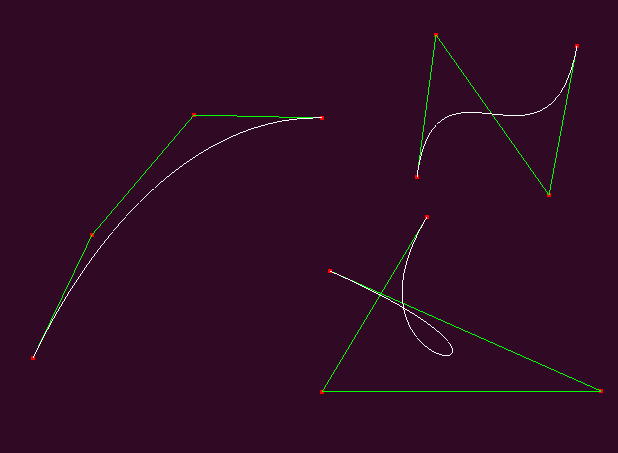
\includegraphics[width=0.5\textwidth, keepaspectratio]{curves.png}
    \caption{Subdivision curves}
    \label{fig:curves}
\end{figure}\\
Previously i forgot to switch the values on the right side, as $R[4]$ is the last point
on the curve, and not the middle one. So the new right side of the reccursion looks like so:
\begin{minted}{cpp}
drawBezierSubdivision(Right[3], Right[2], Right[1], Right[0], ceil(n/2)-1);
\end{minted}
\subsection{Phong Shading}

I am, as previously, using the gl function \emph{glUniform4f} to save
variables from the main code into the \texttt{Fragment Shader}. This enables me to
avoid a some of the very expensive \texttt{Fragment Shader} calculations by moving
it out of the shader functions. This is however only possible on values
that stays constant throughout the fragments, so calculations still has to be
done on \emph{V}, \emph{L} and \emph{R}, as these vectors are dependent on the
position of the current vertex and the current model matrix. \\
These values are pulled out of the \texttt{Vertex Shader} and into the \texttt{Fragment Shader}
using the \emph{varying} keyword, that allows variables to be passed between shaders. 
\begin{minted}{cpp}
static const std::string sVertexShader = "												 
        #version 110                                                                    
                                                                                        
        attribute vec3 aPosition;														
                                                                                        
        uniform mat4 uModelMatrix;														
        uniform mat4 uPerspectiveMatrix;												
                                                                                        
        varying vec4 vPos;              												
        varying mat4 vMat;              												
                                                                                        
        void main() {                                                                   
            vPos = vec4(aPosition.xyz, 1.0);                                            
            vMat = uModelMatrix;                                                        
            gl_Position = uPerspectiveMatrix * uModelMatrix 
                                             * vec4(aPosition.xyz, 1.0);	
        }																				
";

static const std::string sFragmentShader = "														  
        #version 110																	  
                                                                                          
        // from code																	  
        uniform vec4 uAmb, uDif, uSpe, uNormal, uLightPos, uViewPos;	         		  
        uniform int un;																	  
                                                                                          
        // from vertexShader															  
        varying vec4 vPos;                                                                
        varying mat4 vMat;                                                                
                                                                                          
        void main()	{																	  
            vec4 V = normalize(uViewPos * vMat - vPos);                                   
            vec4 L = normalize(uLightPos * vMat - vPos);                                  
            vec4 R = reflect(-L, uNormal);                                                
            gl_FragColor = uAmb + 
                           uDif * dot(L, uNormal) + 
                           uSpe * pow(dot(R, V), un);     
        }																				  
";
\end{minted}
The Phong calculations of all the constants are done in a function called before the patches are drawnn.
The only variable that is calculated on each iteration of the patches is the Normal.
\begin{minted}{cpp}
    Phong(Ia, Ip, Lpos, prp, vrp, Ka, Oa, Kd, Od, Ks, Os, Fatt, n);

    for (int i = 0; i < buffers.size(); i++)
    {
        glm::vec3 Nor = normals.at(i);
        glm::vec3 N = glm::normalize(glm::vec3(Nor[0],Nor[1],Nor[2]));

        gluniform4f(glgetuniformlocation(triangleshaderprogram.getprogram(), 
                    "uNormal"), n[0], n[1], n[2], 1.0);
        buffers.at(i).draw();
    }
\end{minted}
before this code all light variables are declared. the normals are saved in the normals variable, when the buffers are initialized.
the shading can be seen on figures \ref{fig:phongshade}.  

\begin{figure}[h!]
    \centering
    \begin{subfigure}[b]{0.20\textwidth}
        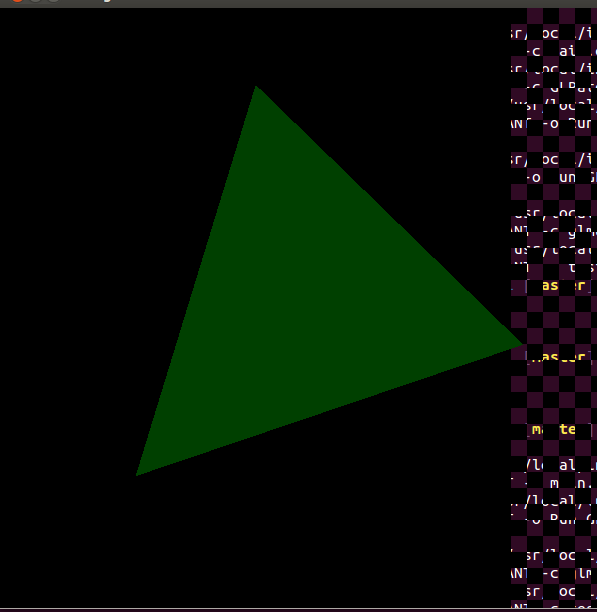
\includegraphics[width=\textwidth, height=2.2cm, keepaspectratio]{amb.png}
        \caption*{Ambient}
        \label{fig:amb}
    \end{subfigure}%
    \begin{subfigure}[b]{0.20\textwidth}
        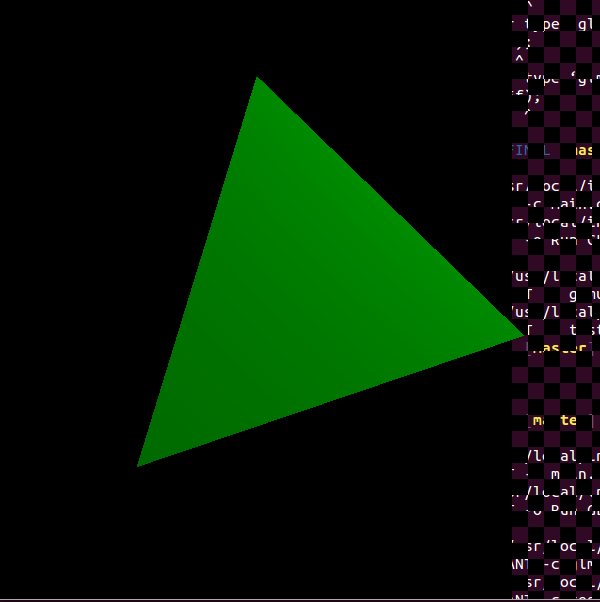
\includegraphics[width=\textwidth, height=2.2cm, keepaspectratio]{dif.png}
        \caption*{Diffusal}
        \label{fig:dif}
    \end{subfigure}
    \begin{subfigure}[b]{0.20\textwidth}
        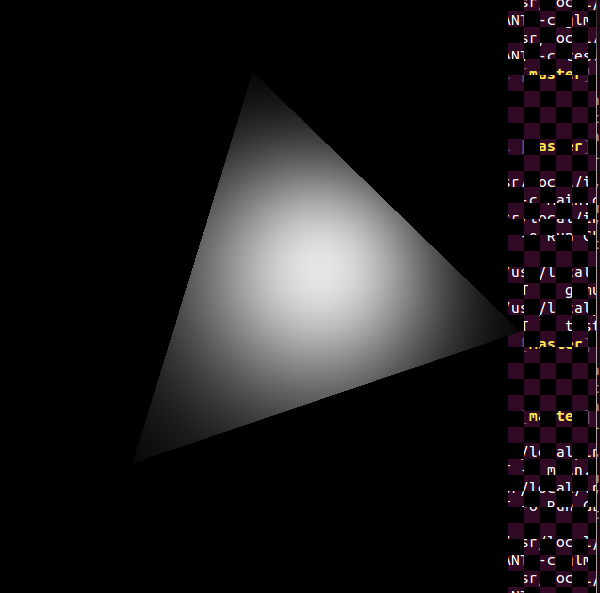
\includegraphics[width=\textwidth, height=2.2cm, keepaspectratio]{spe.png}
        \caption*{Specular}
        \label{fig:spe}
    \end{subfigure}
    \begin{subfigure}[b]{0.20\textwidth}
        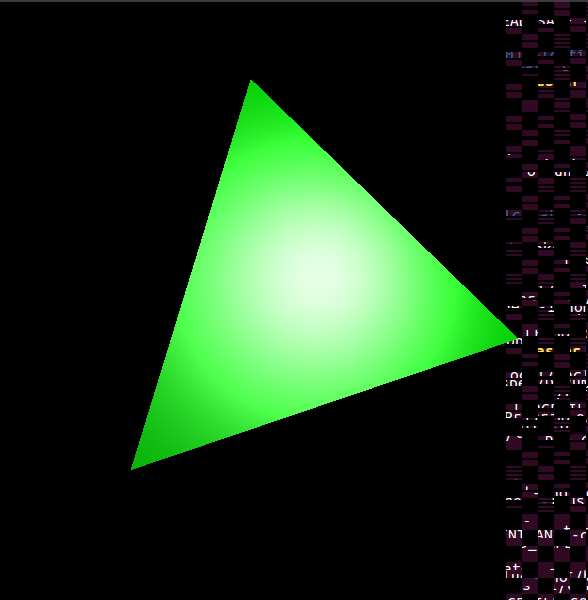
\includegraphics[width=\textwidth, height=2.2cm, keepaspectratio]{all.png}
        \caption*{All}
        \label{fig:all}
    \end{subfigure}
    \caption{Phong Shading}\label{fig:phongshade}
\end{figure}

\end{document}
